% Number of primes in 10^6 consecutive intervals of length 21 starting at 10^9 (bars) against the Poisson law of the same mean 1.013 (dots).
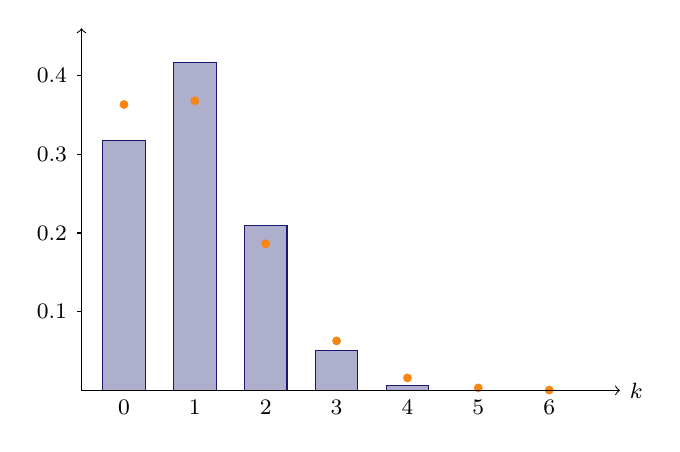
\begin{tikzpicture}[every node/.style={font=\footnotesize}]
\fill[MidnightBlue!35] (-0.270,0) rectangle (0.270,3.170);
\draw[MidnightBlue] (-0.270,0) rectangle (0.270,3.170);
\fill[BurntOrange] (0.000,3.631) circle (1.6pt);
\node[below] at (0.000,0) {$0$};
\fill[MidnightBlue!35] (0.630,0) rectangle (1.170,4.165);
\draw[MidnightBlue] (0.630,0) rectangle (1.170,4.165);
\fill[BurntOrange] (0.900,3.678) circle (1.6pt);
\node[below] at (0.900,0) {$1$};
\fill[MidnightBlue!35] (1.530,0) rectangle (2.070,2.096);
\draw[MidnightBlue] (1.530,0) rectangle (2.070,2.096);
\fill[BurntOrange] (1.800,1.863) circle (1.6pt);
\node[below] at (1.800,0) {$2$};
\fill[MidnightBlue!35] (2.430,0) rectangle (2.970,0.507);
\draw[MidnightBlue] (2.430,0) rectangle (2.970,0.507);
\fill[BurntOrange] (2.700,0.629) circle (1.6pt);
\node[below] at (2.700,0) {$3$};
\fill[MidnightBlue!35] (3.330,0) rectangle (3.870,0.059);
\draw[MidnightBlue] (3.330,0) rectangle (3.870,0.059);
\fill[BurntOrange] (3.600,0.159) circle (1.6pt);
\node[below] at (3.600,0) {$4$};
\fill[MidnightBlue!35] (4.230,0) rectangle (4.770,0.003);
\draw[MidnightBlue] (4.230,0) rectangle (4.770,0.003);
\fill[BurntOrange] (4.500,0.032) circle (1.6pt);
\node[below] at (4.500,0) {$5$};
\fill[MidnightBlue!35] (5.130,0) rectangle (5.670,0.000);
\draw[MidnightBlue] (5.130,0) rectangle (5.670,0.000);
\fill[BurntOrange] (5.400,0.005) circle (1.6pt);
\node[below] at (5.400,0) {$6$};
\draw[->] (-0.540,0)--(6.300,0) node[right] {$k$};
\draw[->] (-0.540,0)--(-0.540,4.600);
\draw (-0.540,1.000)--(-0.600,1.000) node[left] {$0.1$};
\draw (-0.540,2.000)--(-0.600,2.000) node[left] {$0.2$};
\draw (-0.540,3.000)--(-0.600,3.000) node[left] {$0.3$};
\draw (-0.540,4.000)--(-0.600,4.000) node[left] {$0.4$};
\end{tikzpicture}
